
%% bare_jrnl.tex
%% V1.4b
%% 2015/08/26
%% by Michael Shell
%% see http://www.michaelshell.org/
%% for current contact information.B8-85-84-AF-15-1B
%%
%% This is a skeleton file demonstrating the use of IEEEtran.cls
%% (requires IEEEtran.cls version 1.8b or later) with an IEEE
%% journal paper.
%%
%% Support sites: %% http://www.michaelshell.org/tex/ieeetran/
%% http://www.ctan.org/pkg/ieeetran
%% and
%% http://www.ieee.org/

%%*************************************************************************
%% Legal Notice:
%% This code is offered as-is without any warranty either expressed or
%% implied; without even the implied warranty of MERCHANTABILITY or
%% FITNESS FOR A PARTICULAR PURPOSE!
%% User assumes all risk.
%% In no event shall the IEEE or any contributor to this code be liable for
%% any damages or losses, including, but not limited to, incidental,
%% consequential, or any other damages, resulting from the use or misuse
%% of any information contained here.
%%
%% All comments are the opinions of their respective authors and are not
%% necessarily endorsed by the IEEE.
%%
%% This work is distributed under the LaTeX Project Public License (LPPL)
%% ( http://www.latex-project.org/ ) version 1.3, and may be freely used,
%% distributed and modified. A copy of the LPPL, version 1.3, is included
%% in the base LaTeX documentation of all distributions of LaTeX released
%% 2003/12/01 or later.
%% Retain all contribution notices and credits.
%% ** Modified files should be clearly indicated as such, including  **
%% ** renaming them and changing author support contact information. **
%%*************************************************************************


% *** Authors should verify (and, if needed, correct) their LaTeX system  ***
% *** with the testflow diagnostic prior to trusting their LaTeX platform ***
% *** with production work. The IEEE's font choices and paper sizes can   ***
% *** trigger bugs that do not appear when using other class files.       ***                          ***
% The testflow support page is at:
% http://www.michaelshell.org/tex/testflow/



\documentclass[journal]{IEEEtran}
%
% If IEEEtran.cls has not been installed into the LaTeX system files,
% manually specify the path to it like:
% \documentclass[journal]{../sty/IEEEtran}





% Some very useful LaTeX packages include:
% (uncomment the ones you want to load)


% *** MISC UTILITY PACKAGES ***
%
%\usepackage{ifpdf}
% Heiko Oberdiek's ifpdf.sty is very useful if you need conditional
% compilation based on whether the output is pdf or dvi.
% usage:
% \ifpdf
%   % pdf code
% \else
%   % dvi code
% \fi
% The latest version of ifpdf.sty can be obtained from:
% http://www.ctan.org/pkg/ifpdf
% Also, note that IEEEtran.cls V1.7 and later provides a builtin
% \ifCLASSINFOpdf conditional that works the same way.
% When switching from latex to pdflatex and vice-versa, the compiler may
% have to be run twice to clear warning/error messages.






% *** CITATION PACKAGES ***
%
%\usepackage{cite}
% cite.sty was written by Donald Arseneau
% V1.6 and later of IEEEtran pre-defines the format of the cite.sty package
% \cite{} output to follow that of the IEEE. Loading the cite package will
% result in citation numbers being automatically sorted and properly
% "compressed/ranged". e.g., [1], [9], [2], [7], [5], [6] without using
% cite.sty will become [1], [2], [5]--[7], [9] using cite.sty. cite.sty's
% \cite will automatically add leading space, if needed. Use cite.sty's
% noadjust option (cite.sty V3.8 and later) if you want to turn this off
% such as if a citation ever needs to be enclosed in parenthesis.
% cite.sty is already installed on most LaTeX systems. Be sure and use
% version 5.0 (2009-03-20) and later if using hyperref.sty.
% The latest version can be obtained at:
% http://www.ctan.org/pkg/cite
% The documentation is contained in the cite.sty file itself.






% *** GRAPHICS RELATED PACKAGES ***
%
\ifCLASSINFOpdf
  % \usepackage[pdftex]{graphicx}
  % declare the path(s) where your graphic files are
  % \graphicspath{{../pdf/}{../jpeg/}}
  % and their extensions so you won't have to specify these with
  % every instance of \includegraphics
  % \DeclareGraphicsExtensions{.pdf,.jpeg,.png}
\else
  % or other class option (dvipsone, dvipdf, if not using dvips). graphicx
  % will default to the driver specified in the system graphics.cfg if no
  % driver is specified.
  % \usepackage[dvips]{graphicx}
  % declare the path(s) where your graphic files are
  % \graphicspath{{../eps/}}
  % and their extensions so you won't have to specify these with
  % every instance of \includegraphics
  % \DeclareGraphicsExtensions{.eps}
\fi
% graphicx was written by David Carlisle and Sebastian Rahtz. It is
% required if you want graphics, photos, etc. graphicx.sty is already
% installed on most LaTeX systems. The latest version and documentation
% can be obtained at:
% http://www.ctan.org/pkg/graphicx
% Another good source of documentation is "Using Imported Graphics in
% LaTeX2e" by Keith Reckdahl which can be found at:
% http://www.ctan.org/pkg/epslatex
%
% latex, and pdflatex in dvi mode, support graphics in encapsulated
% postscript (.eps) format. pdflatex in pdf mode supports graphics
% in .pdf, .jpeg, .png and .mps (metapost) formats. Users should ensure
% that all non-photo figures use a vector format (.eps, .pdf, .mps) and
% not a bitmapped formats (.jpeg, .png). The IEEE frowns on bitmapped formats
% which can result in "jaggedy"/blurry rendering of lines and letters as
% well as large increases in file sizes.
%
% You can find documentation about the pdfTeX application at:
% http://www.tug.org/applications/pdftex


\usepackage{color}
\usepackage{amsmath}
\usepackage{amssymb}
\usepackage{tabularx}

\usepackage{epsfig}
%\usepackage[colorlinks=false, urlcolor=black, pdfborder={0 0 0}]{hyperref}
%\let\url\nolinkurl
%\usepackage[options]{nohyperref}  % This makes hyperref commands do nothing without errors
\usepackage{url}  % This makes \url work

%\usepackage[dvips]{epsfig}
\usepackage{etoolbox}
\apptocmd{\sloppy}{\hbadness 10000\relax}{}{}

\usepackage{longtable}
\usepackage{graphicx}
\usepackage[T1]{fontenc}
\usepackage{paralist}
\usepackage{enumitem}
%%%%%%%%%%%%for
\usepackage{adjustbox}
\usepackage{array}
\usepackage{booktabs}
\newcolumntype{C}{>{\centering\arraybackslash}X} % centered version of "X" type
\setlength{\extrarowheight}{1pt}
%\usepackage{lipsum}
\usepackage{multirow}

\newcolumntype{R}[2]{%
    >{\adjustbox{angle=#1,lap=\width-(#2)}\bgroup}%
    l%
    <{\egroup}%
}
\newcommand*\rot{\multicolumn{1}{R{90}{1em}}}% no optional argument here, please!

\usepackage{epstopdf}


\def\BibTeX{{\rm B\kern-.05em{\sc i\kern-.025em b}\kern-.08em
    T\kern-.1667em\lower.7ex\hbox{E}\kern-.125emX}}

\usepackage{pdflscape}
%\usepackage{subfigure}
\usepackage{tabularx}
\usepackage{xtab}
%\usepackage{supertabular}

\usepackage{booktabs, threeparttable}
\usepackage{array}
\newcolumntype{L}[1]{>{\raggedright\arraybackslash}p{#1}}

% *** MATH PACKAGES ***
%
%\usepackage{amsmath}
% A popular package from the American Mathematical Society that provides
% many useful and powerful commands for dealing with mathematics.
%
% Note that the amsmath package sets \interdisplaylinepenalty to 10000
% thus preventing page breaks from occurring within multiline equations. Use:
%\interdisplaylinepenalty=2500
% after loading amsmath to restore such page breaks as IEEEtran.cls normally
% does. amsmath.sty is already installed on most LaTeX systems. The latest
% version and documentation can be obtained at:
% http://www.ctan.org/pkg/amsmath





% *** SPECIALIZED LIST PACKAGES ***
%
%\usepackage{algorithmic}
% algorithmic.sty was written by Peter Williams and Rogerio Brito.
% This package provides an algorithmic environment fo describing algorithms.
% You can use the algorithmic environment in-text or within a figure
% environment to provide for a floating algorithm. Do NOT use the algorithm
% floating environment provided by algorithm.sty (by the same authors) or
% algorithm2e.sty (by Christophe Fiorio) as the IEEE does not use dedicated
% algorithm float types and packages that provide these will not provide
% correct IEEE style captions. The latest version and documentation of
% algorithmic.sty can be obtained at:
% http://www.ctan.org/pkg/algorithms
% Also of interest may be the (relatively newer and more customizable)
% algorithmicx.sty package by Szasz Janos:
% http://www.ctan.org/pkg/algorithmicx




% *** ALIGNMENT PACKAGES ***
%
%\usepackage{array}
% Frank Mittelbach's and David Carlisle's array.sty patches and improves
% the standard LaTeX2e array and tabular environments to provide better
% appearance and additional user controls. As the default LaTeX2e table
% generation code is lacking to the point of almost being broken with
% respect to the quality of the end results, all users are strongly
% advised to use an enhanced (at the very least that provided by array.sty)
% set of table tools. array.sty is already installed on most systems. The
% latest version and documentation can be obtained at:
% http://www.ctan.org/pkg/array


% IEEEtran contains the IEEEeqnarray family of commands that can be used to
% generate multiline equations as well as matrices, tables, etc., of high
% quality.




% *** SUBFIGURE PACKAGES ***
%\ifCLASSOPTIONcompsoc
%  \usepackage[caption=false,font=normalsize,labelfont=sf,textfont=sf]{subfig}
%\else
%  \usepackage[caption=false,font=footnotesize]{subfig}
%\fi
% subfig.sty, written by Steven Douglas Cochran, is the modern replacement
% for subfigure.sty, the latter of which is no longer maintained and is
% incompatible with some LaTeX packages including fixltx2e. However,
% subfig.sty requires and automatically loads Axel Sommerfeldt's caption.sty
% which will override IEEEtran.cls' handling of captions and this will result
% in non-IEEE style figure/table captions. To prevent this problem, be sure
% and invoke subfig.sty's "caption=false" package option (available since
% subfig.sty version 1.3, 2005/06/28) as this is will preserve IEEEtran.cls
% handling of captions.
% Note that the Computer Society format requires a larger sans serif font
% than the serif footnote size font used in traditional IEEE formatting
% and thus the need to invoke different subfig.sty package options depending
% on whether compsoc mode has been enabled.
%
% The latest version and documentation of subfig.sty can be obtained at:
% http://www.ctan.org/pkg/subfig




% *** FLOAT PACKAGES ***
%
%\usepackage{fixltx2e}
% fixltx2e, the successor to the earlier fix2col.sty, was written by
% Frank Mittelbach and David Carlisle. This package corrects a few problems
% in the LaTeX2e kernel, the most notable of which is that in current
% LaTeX2e releases, the ordering of single and double column floats is not
% guaranteed to be preserved. Thus, an unpatched LaTeX2e can allow a
% single column figure to be placed prior to an earlier double column
% figure.
% Be aware that LaTeX2e kernels dated 2015 and later have fixltx2e.sty's
% corrections already built into the system in which case a warning will
% be issued if an attempt is made to load fixltx2e.sty as it is no longer
% needed.
% The latest version and documentation can be found at:
% http://www.ctan.org/pkg/fixltx2e


%\usepackage{stfloats}
% stfloats.sty was written by Sigitas Tolusis. This package gives LaTeX2e
% the ability to do double column floats at the bottom of the page as well
% as the top. (e.g., "\begin{figure*}[!b]" is not normally possible in
% LaTeX2e). It also provides a command:
%\fnbelowfloat
% to enable the placement of footnotes below bottom floats (the standard
% LaTeX2e kernel puts them above bottom floats). This is an invasive package
% which rewrites many portions of the LaTeX2e float routines. It may not work
% with other packages that modify the LaTeX2e float routines. The latest
% version and documentation can be obtained at:
% http://www.ctan.org/pkg/stfloats
% Do not use the stfloats baselinefloat ability as the IEEE does not allow
% \baselineskip to stretch. Authors submitting work to the IEEE should note
% that the IEEE rarely uses double column equations and that authors should try
% to avoid such use. Do not be tempted to use the cuted.sty or midfloat.sty
% packages (also by Sigitas Tolusis) as the IEEE does not format its papers in
% such ways.
% Do not attempt to use stfloats with fixltx2e as they are incompatible.
% Instead, use Morten Hogholm'a dblfloatfix which combines the features
% of both fixltx2e and stfloats:
%
% \usepackage{dblfloatfix}
% The latest version can be found at:
% http://www.ctan.org/pkg/dblfloatfix




%\ifCLASSOPTIONcaptionsoff
%  \usepackage[nomarkers]{endfloat}
% \let\MYoriglatexcaption\caption
% \renewcommand{\caption}[2][\relax]{\MYoriglatexcaption[#2]{#2}}
%\fi
% endfloat.sty was written by James Darrell McCauley, Jeff Goldberg and
% Axel Sommerfeldt. This package may be useful when used in conjunction with
% IEEEtran.cls'  captionsoff option. Some IEEE journals/societies require that
% submissions have lists of figures/tables at the end of the paper and that
% figures/tables without any captions are placed on a page by themselves at
% the end of the document. If needed, the draftcls IEEEtran class option or
% \CLASSINPUTbaselinestretch interface can be used to increase the line
% spacing as well. Be sure and use the nomarkers option of endfloat to
% prevent endfloat from "marking" where the figures would have been placed
% in the text. The two hack lines of code above are a slight modification of
% that suggested by in the endfloat docs (section 8.4.1) to ensure that
% the full captions always appear in the list of figures/tables - even if
% the user used the short optional argument of \caption[]{}.
% IEEE papers do not typically make use of \caption[]'s optional argument,
% so this should not be an issue. A similar trick can be used to disable
% captions of packages such as subfig.sty that lack options to turn off
% the subcaptions:
% For subfig.sty:
% \let\MYorigsubfloat\subfloat
% \renewcommand{\subfloat}[2][\relax]{\MYorigsubfloat[]{#2}}
% However, the above trick will not work if both optional arguments of
% the \subfloat command are used. Furthermore, there needs to be a
% description of each subfigure *somewhere* and endfloat does not add
% subfigure captions to its list of figures. Thus, the best approach is to
% avoid the use of subfigure captions (many IEEE journals avoid them anyway)
% and instead reference/explain all the subfigures within the main caption.
% The latest version of endfloat.sty and its documentation can obtained at:
% http://www.ctan.org/pkg/endfloat
%
% The IEEEtran \ifCLASSOPTIONcaptionsoff conditional can also be used
% later in the document, say, to conditionally put the References on a
% page by themselves.




% *** PDF, URL AND HYPERLINK PACKAGES ***
%
%\usepackage{url}
% url.sty was written by Donald Arseneau. It provides better support for
% handling and breaking URLs. url.sty is already installed on most LaTeX
% systems. The latest version and documentation can be obtained at:
% http://www.ctan.org/pkg/url
% Basically, \url{my_url_here}.




% *** Do not adjust lengths that control margins, column widths, etc. ***
% *** Do not use packages that alter fonts (such as pslatex).         ***
% There should be no need to do such things with IEEEtran.cls V1.6 and later.
% (Unless specifically asked to do so by the journal or conference you plan
% to submit to, of course. )


% correct bad hyphenation here
%\hyphenation{op-tical net-works semi-conduc-tor}


\begin{document}
%
% paper title
% Titles are generally capitalized except for words such as a, an, and, as,
% at, but, by, for, in, nor, of, on, or, the, to and up, which are usually
% not capitalized unless they are the first or last word of the title.
% Linebreaks \\ can be used within to get better formatting as desired.
% Do not put math or special symbols in the title.
\title{Fully-Decentralised Reinforcement Learning in Fog-based Internet-of-Things}
%
%
% author names and IEEE memberships
% note positions of commas and nonbreaking spaces ( ~ ) LaTeX will not break
% a structure at a ~ so this keeps an author's name from being broken across
% two lines.
% use \thanks{} to gain access to the first footnote area
% a separate \thanks must be used for each paragraph as LaTeX2e's \thanks
% was not built to handle multiple paragraphs
%

\author{XXX~YYYY,
        and~ XXX~ZZZZ% <-this % stops a space
%\thanks{B. Omoniwa is with National Mathematical Centre, PMB 118, Abuja-Nigeria, email: tunjiomoniwa@gmail.com.}% <-this % stops a space

\thanks{Manuscript received March 14, 2019; revised July X, 2019.}
\thanks{Copyright (c) 2012 IEEE. Personal use of this material is permitted. However, permission to use this material for any other purposes must be obtained from the IEEE by sending a request to pubs-permissions@ieee.org.}
}

% note the % following the last \IEEEmembership and also \thanks -
% these prevent an unwanted space from occurring between the last author name
% and the end of the author line. i.e., if you had this:
%
% \author{....lastname \thanks{...} \thanks{...} }
%                     ^------------^------------^----Do not want these spaces!
%
% a space would be appended to the last name and could cause every name on that
% line to be shifted left slightly. This is one of those "LaTeX things". For
% instance, "\textbf{A} \textbf{B}" will typeset as "A B" not "AB". To get
% "AB" then you have to do: "\textbf{A}\textbf{B}"
% \thanks is no different in this regard, so shield the last } of each \thanks
% that ends a line with a % and do not let a space in before the next \thanks.
% Spaces after \IEEEmembership other than the last one are OK (and needed) as
% you are supposed to have spaces between the names. For what it is worth,
% this is a minor point as most people would not even notice if the said evil
% space somehow managed to creep in.



% The paper headers
\markboth{IEEE Internet of Things Journal,~Vol.~X, No.~X, August~2019}%
{YYYY \MakeLowercase{\textit{et al.}}: Fully-Decentralised Reinforcement Learning in Fog-based Internet-of-Things}
% The only time the second header will appear is for the odd numbered pages
% after the title page when using the twoside option.
%
% *** Note that you probably will NOT want to include the author's ***
% *** name in the headers of peer review papers.                   ***
% You can use \ifCLASSOPTIONpeerreview for conditional compilation here if
% you desire.




% If you want to put a publisher's ID mark on the page you can do it like
% this:
%\IEEEpubid{0000--0000/00\$00.00~\copyright~2015 IEEE}
% Remember, if you use this you must call \IEEEpubidadjcol in the second
% column for its text to clear the IEEEpubid mark.



% use for special paper notices
%\IEEEspecialpapernotice{(Invited Paper)}



% make the title area
\maketitle

% As a general rule, do not put math, special symbols or citations
% in the abstract or keywords.
\begin{abstract}
Reinforcement learning (RL) algorithms offers more insights about the overall futuristic functionalities for intelligent Internet-of-Things (IoT) devices. With the explosive growth in the number of IoT devices, as well as the highly-distributed deployments of these devices today, managing the IoT devices centrally becomes infeasible. As such, several disruptive paradigms have emerged, one of which is the fog computing-based IoT, which aim towards shifting computation, control, and decision-making closer to the network edge. In this paper, we aim to minimize the global outage in communication within a fog-based IoT network, by optimizing the power-control parameter of each potential mobile fog-relay agent (MFRA), as well as optimizing the physical position. As such, each MFRA is compelled to take certain actions that may influence its environment. We optimize the communication performance by applying a decentralized q-learning approach, with each MFRA acting independently, but contributing towards a global optimal policy. Furthermore, we show that our algorithm is scalable even with very large number of devices.

\end{abstract}

% Note that keywords are not normally used for peerreview papers.
\begin{IEEEkeywords}
Reinforcement learning (RL), Internet-of-Things (IoT), Fog-based IoT, Markov decision process (MDP), machine learning (ML).
\end{IEEEkeywords}






% For peer review papers, you can put extra information on the cover
% page as needed:
% \ifCLASSOPTIONpeerreview
% \begin{center} \bfseries EDICS Category: 3-BBND \end{center}
% \fi
%
% For peerreview papers, this IEEEtran command inserts a page break and
% creates the second title. It will be ignored for other modes.
\IEEEpeerreviewmaketitle

\section{Motivation: Idea 1}

For services to be effectively delivered, it is important to ensure that the communication outage within the network is greatly minimized. In Fig. \ref{ideafig1}, we present a scenario where~$n$ number of IoT sensors try to send/receive data/service request to a remote fog device, which has some unique computational/processing capability. Considering the highly-distributed nature of deployed IoT devices, as well as the tendency for increase in the network disruption due to potential obstacles in homes, hospitals, offices, militarised zones, and industries etc., there is a need for some level of intelligence in these devices. In addition to obstacles that obstruct line-of-sight(LOS) communications, the destination device may be to far from the source node, as such, it is possible to leverage fog devices to improve the reliability in the network link. The motivation for this idea was based on some very practical examples, the Industrial IoT (IIoT) and Intelligent monitoring, where industrial robots and surveillance drones could be deployed as relays for meeting stringent quality-of-service(QoS) requirements~\cite{OmoniwaRelay2018}.

\begin{figure}[!t]
\centering
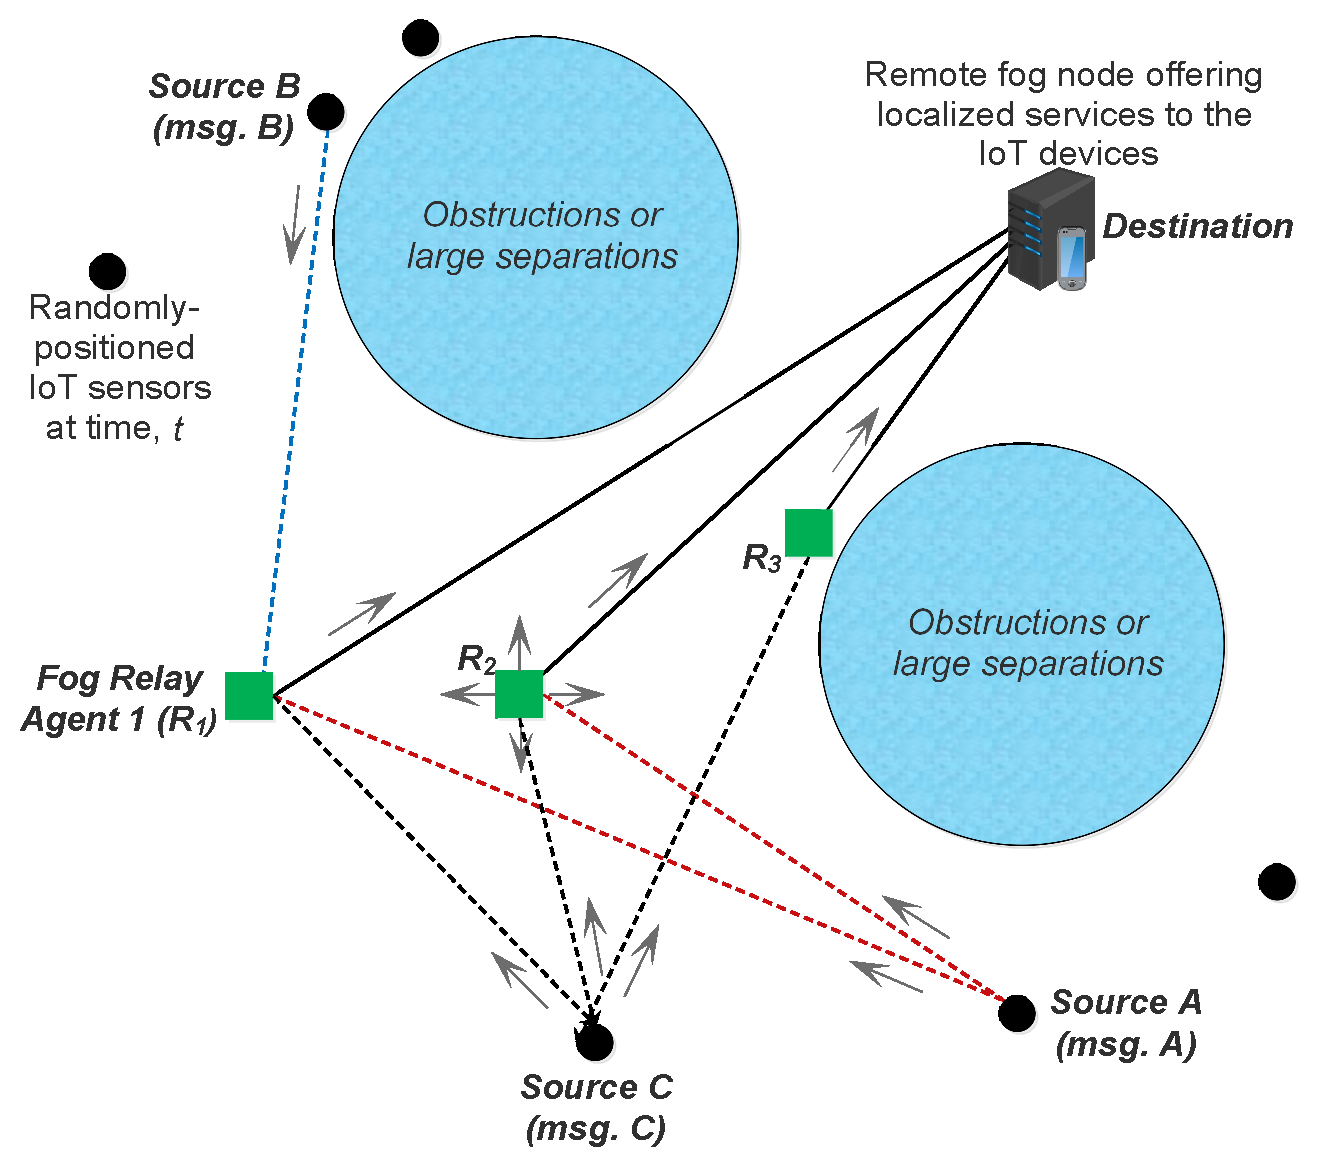
\includegraphics[width=3.2in]{ideafig1.eps}
 %where an .eps filename suffix will be assumed under latex,
% and a .pdf suffix will be assumed for pdflatex; or what has been declared
% via \DeclareGraphicsExtensions.
\caption{System model for Idea1.}
\label{ideafig1}
\end{figure}

\section{Related Works: Idea 1}

Considering the dynamics and heterogeneity within the ultra-distributed IoT environment, it is important for devices which are mobile to move seamlessly without degradation of the quality of service (QoS) when communicating. Moreover, the communication should be ubiquitous irrespective of technology or domain within the system. As such, the RL techniques will play a very important role in areas of IoT device/service discovery, which will support adaptability and interfacing between devices and sub-networks within the IoT domain. Several works in WSNs~\cite{Forster2007}, \cite{Forster2007FROMS}, \cite{Forster2008}, \cite{Forster2009}, focussed on improving some performance metrics such as energy, latency, throughput, within the network.

In \cite{Chen2008}, a reliable and energy-efficient routing (REER) protocol was proposed using a geographic routing approach. The work considered the idea of a central entity, called a reference node (RN), which is assumed to be situated at an ideal location between source and destination. Several other cooperative nodes, which contend to relay data, are assumed to be situated around the RN. The work was able to examine the trade-off between reliability and energy-efficiency when the distances between RNs was adjusted. The work in \cite{Chen2011} proposed an improvement to \cite{Chen2008}, addressing the issue of scalability in a dynamic network. As such, a novel distributed multi-hop cooperative communication scheme (DMC) was proposed to improve certain QoS metrics such as the communication energy, hop count, and end-to-end delay. However, both works assumed complete prior knowledge of the network environment.
In \cite{Liang2009}, a multi-agent reinforcement learning-based multi-hop mesh cooperative (MRL-CC) mechanism for the improvement of some QoS metrics such as the end-to-end delay, packet delivery ratio in the WSNs. The work out-performed the work in \cite{Chen2009}, which incurred higher delay, and was distance-based, which is not suitable for a dynamic network environment. Though the mobility of the cooperative nodes were taken into account when learning the optimal policy, the MRL-CC failed to consider the power dissipated by the power-constrained devices.

A RL-based Q-routing technique, the Feedback Routing for Optimizing Multiple Sinks (FROMS), was proposed in \cite{Forster2007, Forster2007FROMS} to enable efficient routing to multiple sinks without overhead. Simulations were done under scenarios where the sink nodes are mobile and with consideration for node failure. However, the mobility pattern and speed was bounded. Moreover, an important cost metric such as the energy consumed by the mobile nodes was not considered. In \cite{Forster2008}, an evaluation was carried out on the previously proposed FROMS framework using real WSN hardware. The objective was to show that machine learning algorithms could be efficiently deployed on resource-constrained devices. However, during the implementation phase, certain bottlenecks were encountered such as dynamic memory allocation, interference in the wireless channel, poor data gathering, and difficulty in handling lost or corrupted packets. As such, a data clustering and aggregation approach, CLIQUE, was proposed in \cite{Forster2009} to minimize the energy expended by the selecting a cluster head using Q-learning. The approach was able to save significant amount of energy when compared to the traditional and random cluster head selection approach.


Some works~\cite{OmoniwaRelay2018}, \cite{Jadoon2017}, \cite{Camelo2016}, \cite{Li2015} have addressed pertinent issues on cooperative communications within the IoT environment. A Q-learning relay selection algorithm was introduced in \cite{Jadoon2017} to maximize the throughput in a typical cooperative network with relays supporting communication between source and destination. The relays were assumed to be the states, with three possible actions of remaining in the present state with relay~$r$ or choosing~$r + 1$ or~$r - 1$. However, the outage analysis was carried out without a closed-form expression for the outage probability within the network. Furthermore, in an attempt to reduce the complexity of the formulated problem, the problem algorithm did not consider the relays (states) which do not satisfy the minimum mutual information constraint. A scalable parallel Q-learning algorithm was introduced in \cite{Camelo2016} to minimize communication cost. The work considered distributed and resource-constrained environment. A Q-learning-based duty cycle control technique was introduced in \cite{Li2015} to provide improved performance and reliable M2M communication for IoT applications. However, the proposed Q-learning based duty cycle control only considered a two-hop cluster tree network in evaluating the performance of the system. The work in~\cite{OmoniwaRelay2018} built on the concept presented in~\cite{Chiangh2016},  considered a multi-tier fog-based IoT architecture where a mobile/static fog node acts as an amplify and forward relay that transmits received information from a IoT sensor node to a higher hierarchically-placed static fog device, which offers some localized services. An iterative algorithm based on the steepest descent method (SDM) was proposed to jointly optimize the mobility pattern and the transmit power of the fog relay. However, this work the scalability of the approach was not defined. Furthermore, the cost function was unrealistically assumed to be known to the fog relay.

The main task of our work is to minimize global outage in communication within a fog-based IoT network, by optimizing the power-control parameter of the potential mobile fog-relay agent (MFRA), as well as optimizing the position of each relaying agents in the network. As such, each MFRA is compelled to take certain actions that may influence its environment. However, the duration it takes the MFRA to learn is significantly influenced by the state space, as well as the possible set of actions~\cite{Dusparic2009}. The variables for the state, action and reward of an agent may be discrete or continuous, with the former represented as small interval of values which imply distinct levels~\cite{Yau2012}, and can easily be represented in a tabular form. However, it is difficult to represent continuous space using Q-learning tables. The work in \cite{Vucevic2007} considered a RL agent that explores continuous state and action space using Gaussian unit search behaviour. Other works~\cite{Dusparic2009, Cuayahuitl2006} considered the reduction of states by eliminating states that are unlikely to occur. However, this may pose a big risk especially in a highly dynamic environment. RL can be effective for learning action policies in discrete stochastic environments, but its efficiency can decay exponentially with increasing state space~\cite{Uther1998}. Our proposed problem can be observed to have continuous state-action pairs, and is approached by discretizing the state and action space.

It is noteworthy that agents in a multi-agent system (MAS) may take actions that can have direct consequences on neighbouring agents, which may have further impact on other agents within the network. For instance, if a relaying agent decides to increase the transmit power beyond some threshold value, in order to boost its communication capabilities, its action may result in channel interference to its immediate neighbours, and worst, it may deplete its energy fast, and die-out, leading to link failure that can affect the performance of the entire network. Issues like this may arise in a typical multi-agent IoT network, as such, we present a fully-decentralised MAS where each agents learn to follow a local policy that improves the global objective. To the best of our knowledge, this is the first approach that employs a decentralised RL technique to minimize global outage in communication within a fog-based IoT network, taking into consideration the wireless channel conditions, by jointly optimizing the location of each relaying agent and the power-control parameter.

In this paper, we assume the following.
\begin{enumerate}
  \item The MFRA is completely oblivious of its environment, and as such, has no prior knowledge of the overall cost function.
  \item The RN may lower/increase its power level to save energy or increase it to ensure better communication. Also, the MFRA may change its position (2D/3D) depending on the scenario considered.
  \item The MFRA has an objective of learning to make actions that yield better outcomes within its local view of the environment.
  \item The states are be divided into discrete levels to overcome the exponential decay in the efficiency of the proposed approach due infinite state space.
  \item Each MFRA independently tries to optimize power usage and moves in a direction that maximizes the communication outage.
\end{enumerate}





\subsection{Problem Formulation}
In Fig. \ref{ideafig1}, we present a situation where different IoT end-devices, inclusive of smart things embedded with sensors (smart-meters, smart-watches, traffic lights, washing machine, dish-washers, herds, or even a sick patient being monitored, etc.), which can send data/service request to a remote fog service provider via a potential relay node. However, there may be change in the topology of the network or even in the environment, making it difficult for data collection/service provision. Moreover, the environment may be too hazardous for human control. Some level of intelligence is expected from the relay node/agent (RN). The RN learns to optimize its position and adjust it's power-level to minimize the communication outage.

\begin{figure}[!t]
\centering
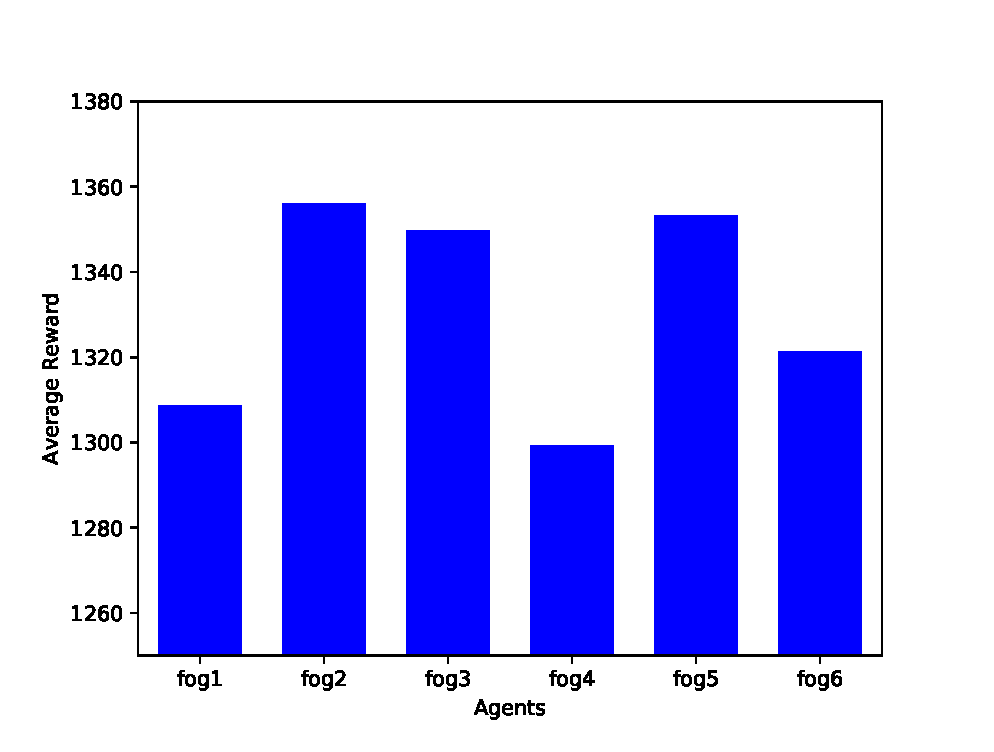
\includegraphics[width=3.1in]{ave_reward.eps}
 %where an .eps filename suffix will be assumed under latex,
% and a .pdf suffix will be assumed for pdflatex; or what has been declared
% via \DeclareGraphicsExtensions.
\caption{Average reward for each agent over 2000 episodes.}
\label{ave_reward}
\end{figure}


\begin{figure}[!t]
\centering
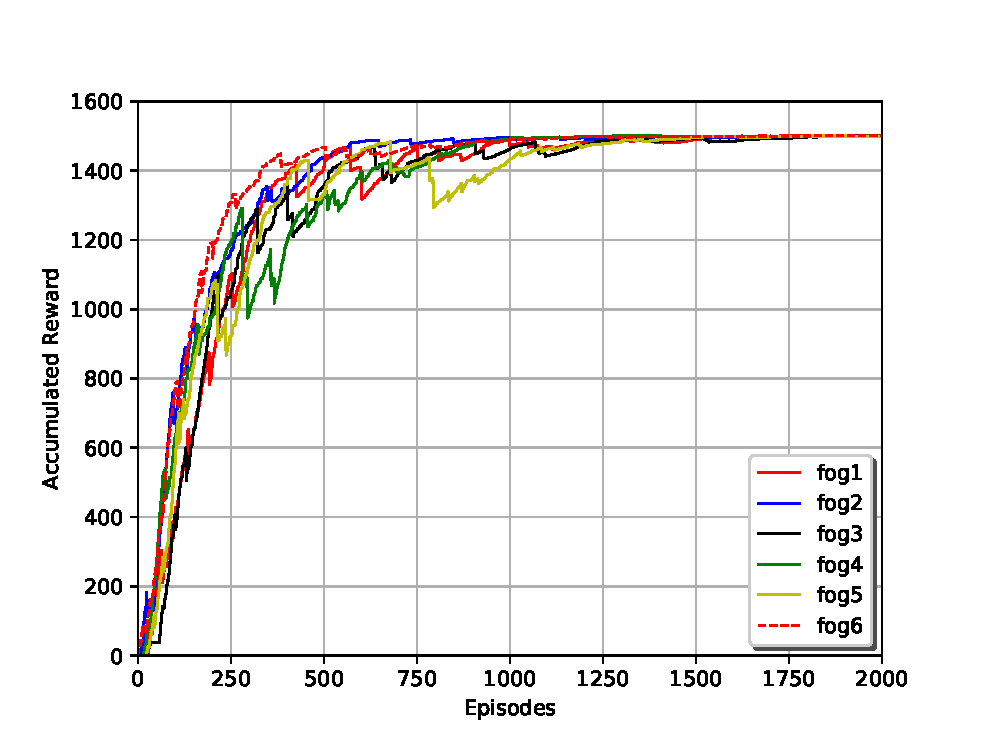
\includegraphics[width=3.1in]{acc_reward.eps}
 %where an .eps filename suffix will be assumed under latex,
% and a .pdf suffix will be assumed for pdflatex; or what has been declared
% via \DeclareGraphicsExtensions.
\caption{Accumulated reward for each agent over 2000 episodes.}
\label{acc_reward}
\end{figure}


\begin{figure}[!t]
\centering
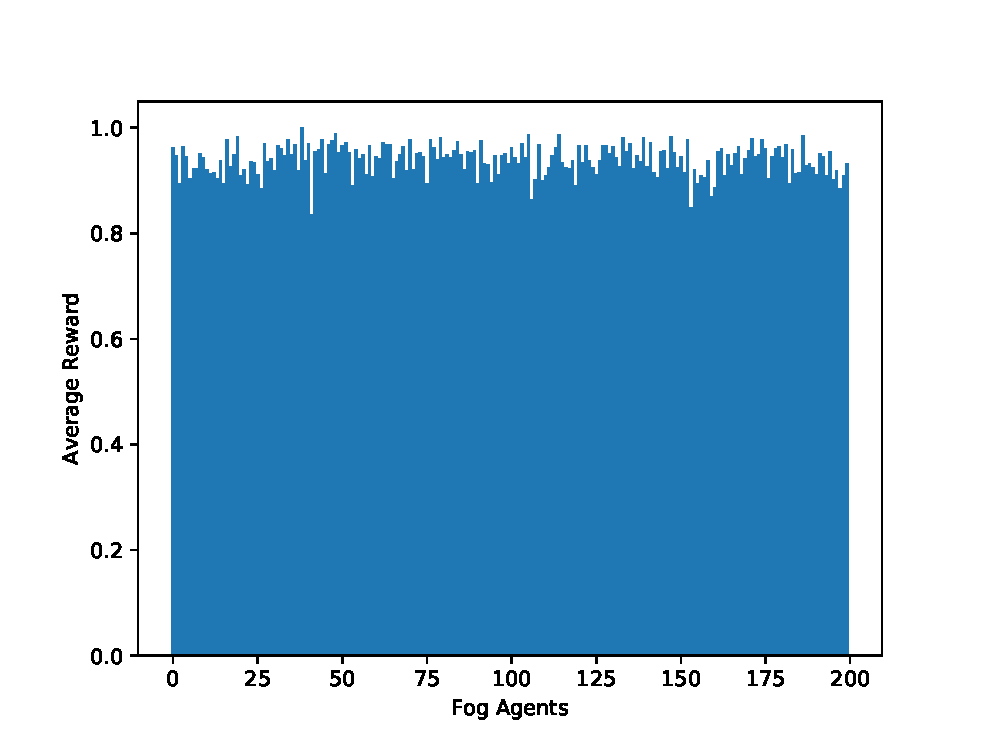
\includegraphics[width=3.1in]{ave_reward_200.eps}
 %where an .eps filename suffix will be assumed under latex,
% and a .pdf suffix will be assumed for pdflatex; or what has been declared
% via \DeclareGraphicsExtensions.
\caption{Average reward for 200 agent over 1000 episodes.}
\label{ave_reward_200}
\end{figure}


\begin{figure}[!t]
\centering
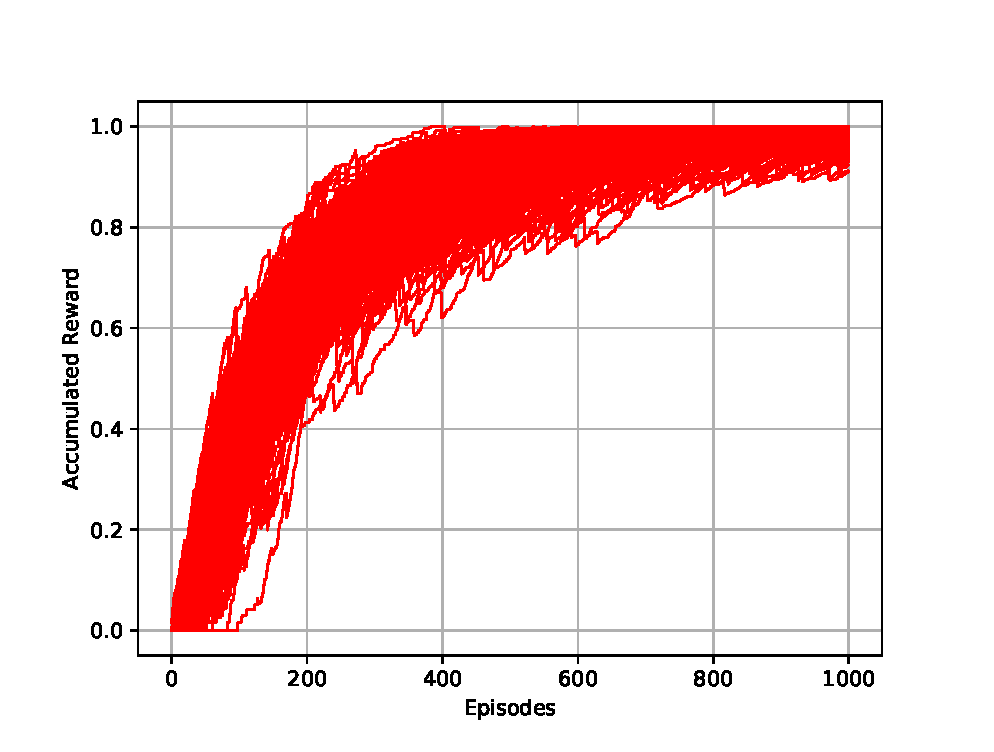
\includegraphics[width=3.1in]{acc_reward_200.eps}
 %where an .eps filename suffix will be assumed under latex,
% and a .pdf suffix will be assumed for pdflatex; or what has been declared
% via \DeclareGraphicsExtensions.
\caption{Accumulated reward for 200 agent over 1000 episodes.}
\label{acc_reward_200}
\end{figure}


\begin{figure}[!t]
\centering
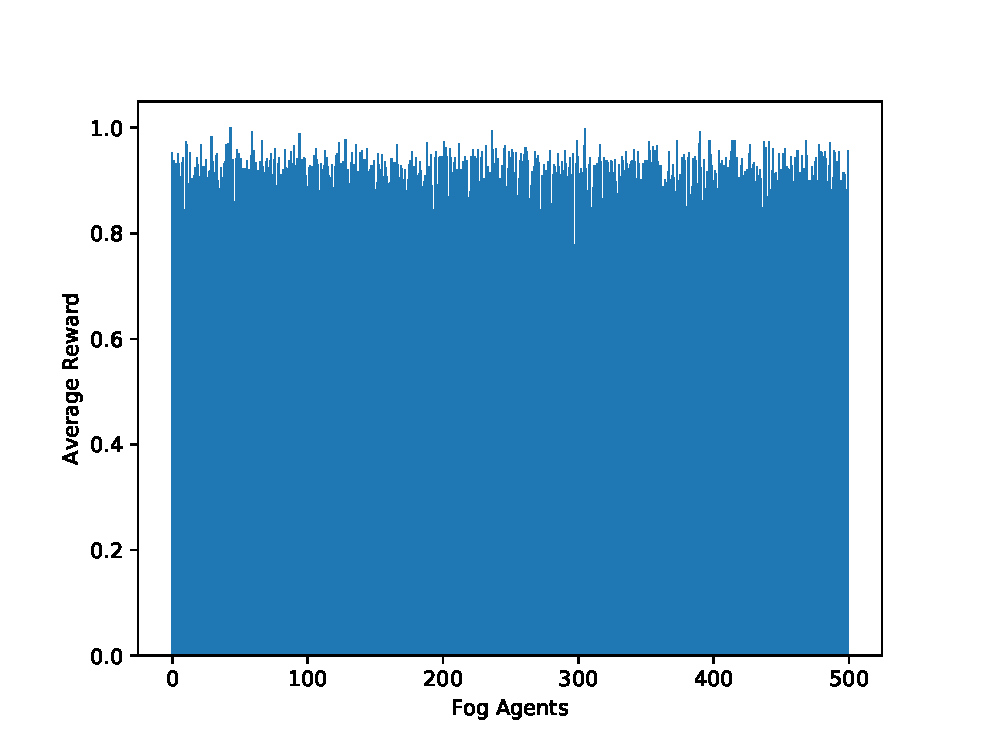
\includegraphics[width=3.1in]{ave_reward_500.eps}
 %where an .eps filename suffix will be assumed under latex,
% and a .pdf suffix will be assumed for pdflatex; or what has been declared
% via \DeclareGraphicsExtensions.
\caption{Average reward for 500 agent over 1000 episodes.}
\label{ave_reward_500}
\end{figure}


\begin{figure}[!t]
\centering
\includegraphics[width=3.1in]{acc_reward_500.eps}
 %where an .eps filename suffix will be assumed under latex,
% and a .pdf suffix will be assumed for pdflatex; or what has been declared
% via \DeclareGraphicsExtensions.
\caption{Accumulated reward for 500 agent over 1000 episodes.}
\label{acc_reward_500}
\end{figure}


\begin{figure}[!t]
\centering
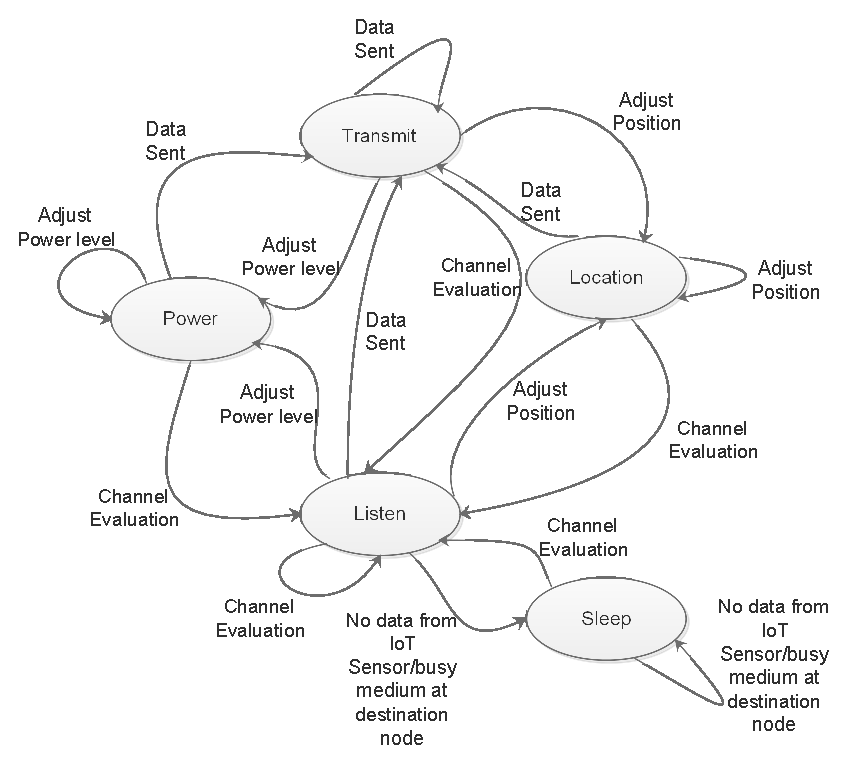
\includegraphics[width=3.2in]{mdp.eps}
 %where an .eps filename suffix will be assumed under latex,
% and a .pdf suffix will be assumed for pdflatex; or what has been declared
% via \DeclareGraphicsExtensions.
\caption{MDP.}
\label{mdp}
\end{figure}

\section{Idea 2}
\label{sec:Idea2a}
\subsection{Problem Formulation}

Devices/agents in an IoT network are resource-constrained, as such, it will be proper to deploy lightweight RL-based techniques that will improve the performance of the network. Furthermore, we may have to experiment on a very dynamic environment considering factors that depict a realistic IoT scenario to meet strict quality-of-service requirements.

In this work, a finite-horizon MDP is considered with continuous state and action spaces defined by the tuple~$\langle \mathcal{S}, \mathcal{A}, p, p_0, \mathcal{P}_{out}, \gamma \rangle$, where~$\mathcal{S}$ is the set of states,~$\mathcal{A}$ is the set of actions,~$p: \mathcal{S}\times \mathcal{A} \times \mathcal{S} \rightarrow \mathbb{G}^+$ is the conditional probability density over successor states given the current state and action,~$p_0: \mathcal{S} \rightarrow \mathbb{G}^+ $ is the probability density over initial states,~$\mathcal{P}_{out}$ is a function that maps state to cost, and the discount factor is~$\gamma \in (0,1]$.
In the RL techniques, the agent has a choice to take certain actions in each time step, causing the environment to respond with new conditions, and consequently, the agent receives reward for that action as a form of feedback. The reward could be positive, negative or even zero, and the main objective of the agent is to maximize the positive reward or minimize the negative reward (often the cost) over the entire time step~$N$.

Our objective is to learn a stochastic policy~$\pi^*: \mathcal{S}\times \mathcal{A}\rightarrow \mathbb{G}^+,$ which is a conditional probability density over the present state, in such a way as to minimize the expected cumulative cost.


\begin{equation}\label{eqn4}
\pi^* = \arg \min_{\pi} \mathbb{E}_{s_0, a_0, s_1, a_1, ..., s_N} \Big[ \sum_{i=0}^{N} \gamma^i \mathcal{P}_{out}(s_i) \Big],
\end{equation}

We take the expectation over the joint distribution of all state-action pairs, with the density give as,

\begin{equation}\label{eqn5}
q(s_0, a_0, s_1, a_1, ..., s_N) = p_0(s_0) \prod_{i=0}^{N-1} \pi(a_i|s_i) p(s_{i+1}|s_i, a_i).
\end{equation}



\begin{figure}[!t]
\centering
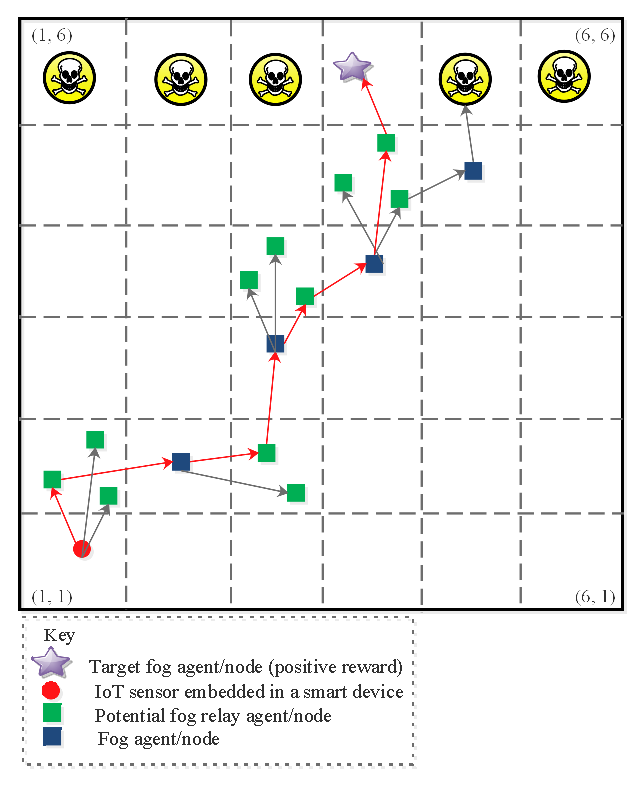
\includegraphics[width=3.2in]{fogmodel2.eps}
 %where an .eps filename suffix will be assumed under latex,
% and a .pdf suffix will be assumed for pdflatex; or what has been declared
% via \DeclareGraphicsExtensions.
\caption{System model depicting the role of fog agents in a dynamic and heterogenous IoT environment with a route policy in red.}
\label{fogmodel2}
\end{figure}

Fig. \ref{fogmodel} shows a dynamic IoT environment with an IoT sensor attempting to request some services from a remote target fog agent/node through randomly deployed fog devices. The devices act as relays to forward traffic from the source to the destination. However, based on their position, line-of-sight(LoS) obstruction, which affect the conditions of the wireless channel, some degree of communication outage may occur. Our aim is to ensure that the agents are able to learn the optimal route to take through their experience with the environment.

\section{Ideas2}\label{sec:Ideas2}

\section{Ideas3}\label{sec:Ideas3}








% use section* for acknowledgment
%\section*{Acknowledgment}
%The authors would like to acknowledge the intellectual and material contributions of COMSATS Institute of Information Technology (CIIT) and The World Academy of Sciences (TWAS) in supporting the Fellowship (FR number: 3240293236).

% Can use something like this to put references on a page
% by themselves when using endfloat and the captionsoff option.
\ifCLASSOPTIONcaptionsoff
  \newpage
\fi

%\newpage

% trigger a \newpage just before the given reference
% number - used to balance the columns on the last page
% adjust value as needed - may need to be readjusted if
% the document is modified later
%\IEEEtriggeratref{8}
% The "triggered" command can be changed if desired:
%\IEEEtriggercmd{\enlargethispage{-5in}}

% references section

% can use a bibliography generated by BibTeX as a .bbl file
% BibTeX documentation can be easily obtained at:
% http://mirror.ctan.org/biblio/bibtex/contrib/doc/
% The IEEEtran BibTeX style support page is at:
% http://www.michaelshell.org/tex/ieeetran/bibtex/
%\bibliographystyle{IEEEtran}
% argument is your BibTeX string definitions and bibliography database(s)
%\bibliography{IEEEabrv,../bib/paper}
%
% <OR> manually copy in the resultant .bbl file
% set second argument of \begin to the number of references
% (used to reserve space for the reference number labels box)
\begin{thebibliography}{1}
\bibitem{Ngu2017}
A. H. Ngu, M. Gutierrez, V. Metsis, S. Nepal and Q. Z. Sheng, "IoT Middleware: A Survey on Issues and Enabling Technologies," in IEEE Internet of Things Journal, vol. 4, no. 1, pp. 1-20, Feb. 2017.

\bibitem{Omoniwa2018}
B. Omoniwa, R. Hussain, M. A. Javed, S. H. Bouk and S. A. Malik, "Fog/Edge Computing-based IoT (FECIoT): Architecture, Applications, and Research Issues," in IEEE Internet of Things Journal.

\bibitem{OmoniwaRelay2018}
B. Omoniwa et al., "An Optimal Relay Scheme for Outage Minimization in Fog-based Internet-of-Things (IoT) Networks," in IEEE Internet of Things Journal.

\bibitem{Chiangh2016}
M. Chiang and T. Zhang, ``Fog and IoT: An Overview of Research Opportuinities,'' IEEE Internet of Things, vol. 3, no. 6, pp. 854-864, Dec.
2016.

\bibitem{Earley2015}
S. Earley, ``Analytics, Machine Learning, and the Internet of Things,'' \emph{IT Professional,} vol. 17, no. 1, pp. 10-13, Jan.-Feb. 2015.

\bibitem{Zhang18}
D. Zhang, X. Han and C. Deng,``Review on the research and practice of deep learning and reinforcement learning in smart grids,'' \emph{CSEE Journal of Power and Energy Systems,} vol. 4, no. 3, pp. 362-370, September 2018.

\bibitem{Watkins92}
C. J. C. H. Watkins and P. Dayan, Machine Learning (1992), Kluwer Academic Publishers, vol. 8: 279.

\bibitem{Wen15}
Z. Wen, D. O'Neill and H. Maei, ``Optimal Demand Response Using Device-Based Reinforcement Learning,'' \emph{IEEE Transactions on Smart Grid,} vol. 6, no. 5, pp. 2312-2324, Sept. 2015.

\bibitem{Sutton98}
R. S. Sutton, and A. G. Barto, \emph{Reinforcement learning - an introduction.} Cambridge, MA: MIT Press, 1998.

\bibitem{Jadoon2017}
M. A. Jadoon and S. Kim, "Relay selection Algorithm for wireless cooperative networks: a learning-based approach," in IET Communications, vol. 11, no. 7, pp. 1061-1066, 11 5 2017.

\bibitem{Zhu2018}
J. Zhu, Y. Song, D. Jiang and H. Song, ``A New Deep-Q-Learning-Based Transmission Scheduling Mechanism for the Cognitive Internet of Things,'' \emph{IEEE Internet of Things Journal,} vol. 5, no. 4, pp. 2375-2385, Aug. 2018.

\bibitem{Zhu2013}
J. Zhu, Z. Peng and F. Li, ``A transmission and scheduling scheme based on W-learning algorithm in wireless networks,'' \emph{2013 8th International Conference on Communications and Networking in China (CHINACOM),} Guilin, 2013, pp. 85-90.

\bibitem{Gai2018}
K. Gai, M. Qiu, ``Optimal resource allocation using reinforcement learning for IoT content-centric services,'' \emph{Applied Soft Computing,} vol. 70,
pp. 12-21, Sept. 2018.

\bibitem{Dusparic2009}
I. Dusparic and V. Cahill, ``Distributed W-Learning: Multi-Policy Optimization in Self-Organizing Systems,'' 2009 Third IEEE International Conference on Self-Adaptive and Self-Organizing Systems, San Francisco, CA, 2009, pp. 20-29.

\bibitem{Zhou2018}
L. Zhou, A. Swain and A. Ukil, ``Q-learning and Dynamic Fuzzy Q-learning Based Intelligent Controllers for Wind Energy Conversion Systems,'' \emph{2018 IEEE Innovative Smart Grid Technologies - Asia (ISGT Asia),} Singapore, 2018, pp. 103-108.

\bibitem{Park2016}
T. Park, N. Abuzainab and W. Saad, ``Learning How to Communicate in the Internet of Things: Finite Resources and Heterogeneity,'' \emph{IEEE Access,} vol. 4, pp. 7063-7073, 2016.

\bibitem{Hans2010}
A. Hans and S. Udluft, ``Ensembles of Neural Networks for Robust Reinforcement Learning,'' \emph{2010 Ninth International Conference on Machine Learning and Applications,} Washington, DC, 2010, pp. 401-406.

\bibitem{Nguyen2017}
D. D. Nguyen, H. X. Nguyen and L. B. White, ``Reinforcement Learning With Network-Assisted Feedback for Heterogeneous RAT Selection,'' \emph{IEEE Transactions on Wireless Communications,} vol. 16, no. 9, pp. 6062-6076, Sept. 2017.

\bibitem{Mohammadi2018}
M. Mohammadi, A. Al-Fuqaha, M. Guizani and J. Oh, ``Semisupervised Deep Reinforcement Learning in Support of IoT and Smart City Services,'' \emph{IEEE Internet of Things Journal,} vol. 5, no. 2, pp. 624-635, April 2018.

\bibitem{Alletto2016}
S. Alletto et al., ``An Indoor Location-Aware System for an IoT-Based Smart Museum,'' \emph{IEEE Internet of Things Journal,} vol. 3, no. 2, pp. 244-253, April 2016.
doi: 10.1109/JIOT.2015.2506258

\bibitem{Kolomvatsos2017}
K. Kolomvatsos, and C. Anagnostopoulos, ``Reinforcement Learning for Predictive Analytics in
Smart Cities,'' \emph{Informatics,} vol. 3, no. 16, June 2017.

\bibitem{Conti2017}
S. Conti, G. Faraci, R. Nicolosi, S. A. Rizzo and G. Schembra, ``Battery Management in a Green Fog-Computing Node: a Reinforcement-Learning Approach,'' \emph{IEEE Access,} vol. 5, pp. 21126-21138, 2017.

\bibitem{Mai2018}
L. Mai, N.-N. Dao, and M. Park, ``Real-time task assignment approach leveraging reinforcement learning with evolution strategies for long-term latency minimization in fog computing,'' \emph{Sensors,} vol. 18, no. 2830, Aug. 2018.

\bibitem{Kwok2004}
C. Kwok and D. Fox, ``Reinforcement learning for sensing strategies,'' \emph{2004 IEEE/RSJ International Conference on Intelligent Robots and Systems (IROS) (IEEE Cat. No.04CH37566),} Sendai, 2004, pp. 3158-3163 vol.4.

\bibitem{Li2015}
Y. Li, K. K. Chai, Y. Chen and J. Loo, ``Smart duty cycle control with reinforcement learning for machine to machine communications,'' \emph{2015 IEEE International Conference on Communication Workshop (ICCW),} London, 2015, pp. 1458-1463.

\bibitem{Li2014}
Y. Li, K. K. Chai, Y. Chen and J. Loo, ``Optimised delay-energy aware duty cycle control for IEEE 802.15.4 with cumulative acknowledgement,'' \emph{2014 IEEE 25th Annual International Symposium on Personal, Indoor, and Mobile Radio Communication (PIMRC),} Washington, DC, 2014, pp. 1051-1056.

\bibitem{Grammatopoulou2018}
M. Grammatopoulou, A. Kanellopoulos, and K. G. Vamvoudakis, ``A multi-step and resilient predictive Q-learning algorithm for IoT: a case study in water supply networks'', \emph{ACM Proceedings of the 8th International Conference on the Internet of Things,} Santa Barbara, California, 2018, pp. 1-8.

\bibitem{Debizet2018}
Y. Debizet, G. Lallement, F. Abouzeid, P. Roche and J. Autran, "Q-Learning-based Adaptive Power Management for IoT System-on-Chips with Embedded Power States," 2018 IEEE International Symposium on Circuits and Systems (ISCAS), Florence, 2018, pp. 1-5.

\bibitem{Khan2018}
M. I. Khan, M. M. Alam, Y. Le Moullec and E. Yaacoub, "Cooperative reinforcement learning for adaptive power allocation in device-to-device communication," 2018 IEEE 4th World Forum on Internet of Things (WF-IoT), Singapore, 2018, pp. 476-481.

\bibitem{routray2017}
S. K. Routray and Sharmila K. P., ``Routing in dynamically changing node location scenarios: A reinforcement learning approach,'' 2017 Third International Conference on Advances in Electrical, Electronics, Information, Communication and Bio-Informatics (AEEICB), Chennai, 2017, pp. 458-462.

\bibitem{Liu2017}
Y. Liu, L. Liu and W. Chen, "Intelligent traffic light control using distributed multi-agent Q learning," 2017 IEEE 20th International Conference on Intelligent Transportation Systems (ITSC), Yokohama, 2017, pp. 1-8.

\bibitem{Dias2016}
G. M. Dias, M. Nurchis and B. Bellalta, "Adapting sampling interval of sensor networks using on-line reinforcement learning," 2016 IEEE 3rd World Forum on Internet of Things (WF-IoT), Reston, VA, 2016, pp. 460-465.

\bibitem{Camelo2016}
M. Camelo and J. F. a. S. Latré, "A Scalable Parallel Q-Learning Algorithm for Resource Constrained Decentralized Computing Environments," 2016 2nd Workshop on Machine Learning in HPC Environments (MLHPC), Salt Lake City, UT, 2016, pp. 27-35.

\bibitem{Nassar}
A. T. Nassar, and Y. Yilmaz, ``Reinforcement-Learning-Based Resource Allocation in Fog Radio Access Networks for Various IoT Environments,'' Arxiv

%%%%%%%%%%%%%%WSN
\bibitem{Chen2008}
M. Chen, T. Kwon, S. Mao, Y. Yuan and V. C. M. Leung, ``Reliable and energy-efficient routing protocol in dense wireless sensor networks,'' Int. J. Sen. Netw.
 vol. 4, no. 1/2, pp. 104-117, July 2008.

\bibitem{Chen2011}
M. Chen, M. Qiu, L. Liao, J. Park and J. Ma, ``Distributed multi-hop cooperative communication in dense wireless sensor networks'', \emph{The Journal of Supercomputing,} vol. 56, no. 3, pp. 353-369, June 2011.

\bibitem{Liang2009}
Xuedong Liang, Min Chen, Yang Xiao, I. Balasingham and V. C. M. Leung, ``A novel cooperative communication protocol for QoS provisioning in wireless sensor networks,'' 2009 5th International Conference on Testbeds and Research Infrastructures for the Development of Networks and Communities and Workshops, Washington, DC, 2009, pp. 1-6.

\bibitem{Chen2009}
M. Chen, Xuedong Liang, V. Leung and I. Balasingham, "Multi-hop mesh cooperative structure based data dissemination for wireless sensor networks," 2009 11th International Conference on Advanced Communication Technology, Phoenix Park, 2009, pp. 102-106.

\bibitem{Mihaylov}
M. Mihaylov and Y. L. Borgne, ``Decentralised reinforcement learning for energy-efficient scheduling in wireless sensor networks,'' Int. J. Communication Networks and Distributed Systems, Vol. 9, Nos. 3/4, 2012

\bibitem{Shah2007}
K. Shah and M. Kumar, ``Distributed Independent Reinforcement Learning (DIRL) Approach to Resource Management in Wireless Sensor Networks,'' 2007 IEEE International Conference on Mobile Adhoc and Sensor Systems, Pisa, 2007, pp. 1-9.

\bibitem{Shah2013}
K. Shah, M. D. Francesco and M. Kumar, ``Distributed resource management in wireless sensor networks using reinforcement learning,'' Wireless Networks,
vol. 19, no. 5, pp. 705-724, July 2013.

\bibitem{Yau2012}
K.-L. A. Yau, P. Komisarczuk, P. D. Teal, ``Reinforcement learning for context awareness and intelligence in wireless
networks: Review, new features and open issues,'' Journal of Network and Computer Applications, vol. 35, no. 1, pp. 253-267, Jan. 2012.

\bibitem{Yau2015}
K.-L. A. Yau, H. G. Goh, D. Chieng and K. H. Kwong, ``Application of reinforcement learning to wireless sensor networks: models and algorithms,'' Computing, vol. 97, no. 11, pp. 1045–1075, Nov. 2015.

\bibitem{Forster2007}
A. Egorova-Forster and A. L. Murphy, "Exploiting Reinforcement Learning for Multiple Sink Routing in WSNs," 2007 IEEE International Conference on Mobile Adhoc and Sensor Systems, Pisa, 2007, pp. 1-3.

\bibitem{Forster2007FROMS}
A. Forster and A. L. Murphy, "FROMS: Feedback Routing for Optimizing Multiple Sinks in WSN with Reinforcement Learning," 2007 3rd International Conference on Intelligent Sensors, Sensor Networks and Information, Melbourne, Qld., 2007, pp. 371-376.

\bibitem{Forster2008}
A. Forster, A. L. Murphy, J. Schiller and K. Terfloth, "An Efficient Implementation of Reinforcement Learning Based Routing on Real WSN Hardware," 2008 IEEE International Conference on Wireless and Mobile Computing, Networking and Communications, Avignon, 2008, pp. 247-252.

\bibitem{Forster2009}
A. Forster and A. L. Murphy, "CLIQUE: Role-Free Clustering with Q-Learning for Wireless Sensor Networks," 2009 29th IEEE International Conference on Distributed Computing Systems, Montreal, QC, 2009, pp. 441-449.

\bibitem{Vucevic2007}
N. Vucevic, J. Perez-Romero, O. Sallent and R. Agusti, "Reinforcement Learning for Active Queue Management in Mobile All-IP Networks," 2007 IEEE 18th International Symposium on Personal, Indoor and Mobile Radio Communications, Athens, 2007, pp. 1-5.

\bibitem{Uther1998}
W. T. B. Uther and M. M. Veloso, ``Tree Based Discretization for Continuous State Space Reinforcement Learning,'' \emph{Proceedings of the Fifteenth National/Tenth Conference on Artificial Intelligence/Innovative Applications of Artificial Intelligence,} 1998, Madison, Wisconsin, USA, pp. 769-774.

\bibitem{Cuayahuitl2006}
H. Cuayahuitl, S. Renals, O. Lemon, and H. Shimodaira. ``Learning multi-goal dialogue strategies using reinforcement learning with reduced state-action spaces,'' In Int. Journal of Game Theory, pp. 547–565, 2006.
\end{thebibliography}


% that's all folks
\end{document}


